\chapter{Espaces de Lebesgue}
\begin{abstract}
Les espaces~$L^p$ sont indispensables à la définition des espaces de Sobolev après
lesquels nous courons depuis quelques chapitres.

La mesure de Lebesgue a été introduite, les notions d'application et
de continuité ont été rappelées... nous en avons plus qu'il ne nous en faut
pour définir de tels espaces.
\end{abstract}
Comme promis au paragraphe~\ref{Sec-impasse}, nous fournissons maintenant quelques compléments sur l'intégration. Nous avons mentionné la mise en défaut de l'intégrale de Riemann\index[aut]{Riemann (Georg Friedrich Bernhard), 1826-1866, Allemand} dans le cas de l'indicatrice des rationnels.
Ce contre-exemple a été historiquement fourni par Dirichlet.\index[aut]{Dirichlet (Johann Peter Gustav Lejeune), 1805-1859, Allemand}
Regardons toutefois d'un peu plus près d'où tout cela provient.

\medskip
\begin{histoire}%
Dans le chapitre VI, «Développement d'une fonction arbitraire en séries trigonométriques» de sa \emph{Théorie analytique}, Fourier\index[aut]{Fourier (Jean Baptiste Joseph), 1768-1830, Français} considère une fonction~$f$ définie dans~$]-\pi/2,+\pi/2[$ dont le développement en série trigonométrique est de la forme:
\begin{equation} f(x)=a_1\sin x+a_2\sin 2x +\ldots+a_k\sin kx +\ldots\end{equation}
\sbox{\MaBoiteAvecPhotos}{\setlength{\tabcolsep}{0pt}\scriptsize%
\begin{tabular}{c}%
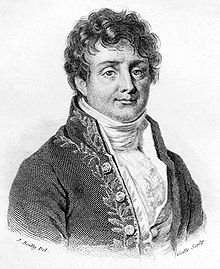
\includegraphics[height=\the\HauteurDesPhotos]{Fourier}\\
Fourier%
\end{tabular}}
\medskip
\ImageAGauche{%
Le problème est de calculer les coefficients~$a_k$ dans le cas même, dit-il, où «la fonction~$f(x)$ représente une suite de valeurs ou ordonnées dont chacune est arbitraire... On ne suppose point que ces coordonnées soient assujetties à une loi commune; elles se succèdent d'une manière quelconque et chacune d'elles est donnée comme le serait une seule quantité».\\ \indent
On notera au passage que la fonction considérée par Fourier\index[aut]{Fourier (Jean Baptiste Joseph), 1768-1830, Français} n'est définie que par la donnée de ses points (si en plus ils sont en nombre fini, cela représente alors un échantillonnage).\\ \indent
%
%\medskip
Fourier\index[aut]{Fourier (Jean Baptiste Joseph), 1768-1830, Français} conduit son calcul selon une voie nouvelle: en multipliant l'expression précédente par~$\sin kx$ et en intégrant terme à terme la série, mais sans justification, il obtient:
\begin{equation}a_k=\frac2{\pi}\dint_0^{\pi} f(x)\sin kx \dd x\end{equation}
Fourier\index[aut]{Fourier (Jean Baptiste Joseph), 1768-1830, Français} observe que dans tous les cas envisagés, ces intégrales ont un sens et en conclut que toute fonction d'une variable peut-être représentée par une série trigonométrique.}

Fourier,\index[aut]{Fourier (Jean Baptiste Joseph), 1768-1830, Français} même manquant de rigueur, aboutit à un résultat juste pour les fonctions qu'il considère.
Or les fonctions considérées en l'occurrence «vont bien» pour l'intégrale de Riemann\index[aut]{Riemann (Georg Friedrich Bernhard), 1826-1866, Allemand} telle qu'elle est définie.

\medskip
\index[aut]{Riemann (Georg Friedrich Bernhard), 1826-1866, Allemand}
\begin{definition}[Intégrale de Riemann]
Soit~$f$ une fonction réelle définie sur un intervalle~$\intff{a}{b}$.
On considère une suite~$(x_i)$, $0\le i\le n$ de subdivisions de cet intervalle:
$a=x_0 < x_1 <\ldots < x_{n-1} <x_n=b$.
Notons~$\delta_i=x_i-x_{i-1}$ et~$S=\delta_1f(a+\varepsilon_1\delta_1) +
\delta_2 f(x_1+\varepsilon_2\delta_2)+ \ldots + \delta_nf(x_{n-1}+\varepsilon_n\delta_n)$,
où~$0\le \delta_i\le 1$.

Si la somme~$S$ a la propriété, de quelque manière que les~$\delta$ et les
$\varepsilon$ puissent être choisis, de s'approcher indéfiniment d'une limite fixe~$A$,
quand les~$\delta$ tendent vers zéro, cette limite s'appelle la valeur de l'intégrale
définie~$\int_a^b f(x)\dd x$.
\end{definition}
En termes modernes, on dira que pour qu'une fonction bornée soit Riemann-intégrable,\index[aut]{Riemann (Georg Friedrich Bernhard), 1826-1866, Allemand}
il faut et il suffit que l'ensemble des points de discontinuité de~$f$ soit de mesure nulle.
\textcolorgris{En complément, on rappelera également que l'intégrale de Riemann n'est que la généralisation
de celle de Cauchy:\index[aut]{Cauchy (Augustin Louis, baron -), 1789-1857, Français} la valeur retenue pour calculer
la fonction sur chaque sous-intervalle n'est plus celle du point de gauche, mais peut être prise n'importe où dans ledit sous-intervalle.}

\sbox{\MaBoiteAvecPhotos}{\setlength{\tabcolsep}{0pt}\scriptsize%
\begin{tabular}{ccc}%
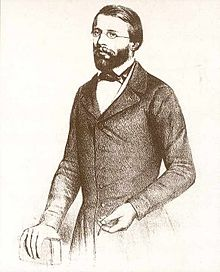
\includegraphics[height=\the\HauteurDesPhotos]{Riemann}&
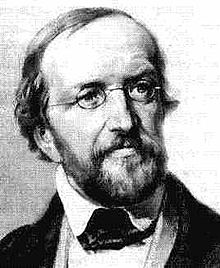
\includegraphics[height=\the\HauteurDesPhotos]{Dirichlet}&
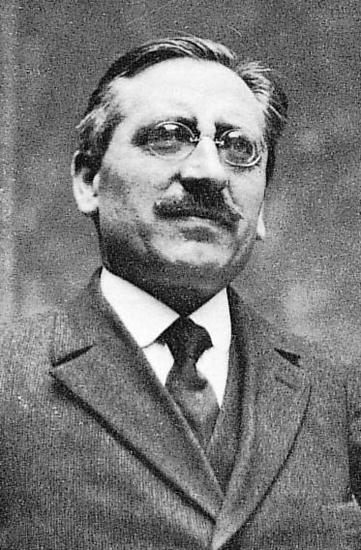
\includegraphics[height=\the\HauteurDesPhotos]{Lebesgue2}\\
Riemann&Dirichlet&Lebesgue%
\end{tabular}}
\medskip
\ImageADroite{%
Dès la fin de son mémoire de 1829, \emph{Sur la convergence des séries trigonométriques qui servent à représenter une fonction arbitraire entre des limites données}, Dirichlet\index[aut]{Dirichlet (Johann Peter Gustav Lejeune), 1805-1859, Allemand} donne l'exemple, d'une nature toute nouvelle, d'une fonction discontinue en tous ces points: la fonction~$f(x)$ qui vaut une constante~$c$ si~$x$ est un rationnel et qui vaut une autre constante~$d$ si~$x$ est irrationnel.
On voit alors directement que la Riemann-intégrabilité est mise à mal.\index[aut]{Riemann (Georg Friedrich Bernhard), 1826-1866, Allemand} Le travail consistera alors à définir précisément ce que l'on peut négliger, i.e. les parties de mesure nulle.
}

\medskip
Lebesgue\index[aut]{Lebesgue (Henri-Léon), 1875-1941, Français} va commencer par définir un \textcolorblue{ensemble mesurable}: c'est un ensemble dont la mesure extérieure (i.e. la borne inférieure de la mesure des ouverts le contenant) est égale à sa mesure intérieure (i.e. la borne supérieure de la mesure des fermés qu'il contient): est-il besoin de rappeler la différence entre borne inférieure et minimum et entre borne supérieure et maximum ? La borne supérieure (ou le supremum) d'une partie d'un ensemble partiellement ordonné est le plus petit de ses majorants. Une telle borne n'existe pas toujours, mais si elle existe alors elle est unique. Elle n'appartient pas nécessairement à la partie considérée.
Dualement, la borne inférieure (ou l'infimum) d'une partie est le plus grand de ses minorants...

\textcolorblue{L'intégrale de Lebesgue}\index[aut]{Lebesgue (Henri-Léon), 1875-1941, Français} peut être définie de manière géométrique: pour une fonction positive~$f$ définie sur~$\intff{a}{b}$, elle est égale à la mesure de dimension deux de l'ensemble $\{(x,y)\in\RR^2 / a\le y\le f(x), a\le x\le b\}$ quand cette mesure existe.
D'une manière analytique, cette définition de l'intégrale de Lebesgue devient:\index[aut]{Lebesgue (Henri-Léon), 1875-1941, Français}

\begin{definition}[Intégrale de Lebesgue]
soit~$f$ une fonction réelle, bornée, définie sur~$\intff{a}{b}$.
Supposons~$m\le f(x)\le M$ pour~$x\in\intff{a}{b}$.
Pour tous~$\xi, \eta$ tels que~$\xi\le\eta$, on définit:
$V_{\xi,\eta}=\{x\in\intff{a}{b}/ \xi\le f(x)\le\eta\}$.
Si pour tous~$\xi$, $\eta$, $V_{\xi,\eta}$ est mesurable, alors~$f$ est mesurable.

En considérant la partition~$m=\xi_1<\xi_2<...<\xi_n<\xi_{n+1}=M$ et
$V_i=\{x/ \xi_i\le f(x)\le\xi_{i+1}\}$, on définit les sommes
\begin{equation} \dsum_{i=1}^n\xi_i m(V_i) \quad \text{ et }\quad \dsum_{i=1}^n\xi_{i+1} m(V_i) \end{equation}
où~$m(V)$ est la mesure de l'ensemble~$V$.
\textcolorblue{L'intégrale de Lebesgue}\index[aut]{Lebesgue (Henri-Léon), 1875-1941, Français} est la \textcolorblue{limite commune} de ces deux sommes, dont on peut montrer qu'elle existe lorsque~$f$ est mesurable.
\end{definition}

%\medskip
Voici par quelle image Lebesgue\index[aut]{Lebesgue (Henri-Léon), 1875-1941, Français} expliquait la nature de son intégrale:\\
«Je dois payer une certaine somme; je fouille dans mes poches et j'en sors des pièces et des billets de différentes valeurs. Je les verses à mon créancier dans l'ordre où elles se présentent jusqu'à atteindre le total de ma dette. C'est l'intégrale de Riemann.\index[aut]{Riemann (Georg Friedrich Bernhard), 1826-1866, Allemand} Mais je peux opérer autrement. Ayant sorti tout mon argent, je réunis les billets de même valeur, les pièces semblables et j'effectue le paiement en donnent ensemble les signe monétaires de même valeur. C'est mon intégrale.»

\medskip
La théorie de Lebesgue\index[aut]{Lebesgue (Henri-Léon), 1875-1941, Français} éclaire bien des difficultés des discussions du \textsc{xix}\fup{e} siècle (notamment sur les propriétés de différentiabilité des fonctions continues) et fournit un cadre général simplifié à de nombreux théorèmes alors que la théorie de Riemann\index[aut]{Riemann (Georg Friedrich Bernhard), 1826-1866, Allemand} multiplie les hypothèses et les conditions restrictives.

De plus, toute cette évolution s'est accompagnée de l'idée qu'on doit manipuler les fonctions comme des objets mathématiques en soi, des points de nouveaux espaces, les \emph{espaces fonctionnels}. Avec l'extension du langage ensembliste, il devient naturel d'employer un langage géométrique à propos de ces espaces.

\medskip
\textcolorgris{Malgré tout ce qui vient d'être dit, rendons quand même hommage à cette belle (et malgré tout puissante) intégrale de Riemann, qui a de plus le bon goût d'être souvent très bien comprise des élèves.\\ \indent
L'intégrale de Riemann nous apprend à nous poser la question «où se passent les choses importantes?», question qui n'a pas de sens pour l'intégrale de Lebesgue qui ne connaît pas la question «où?», mais seulement «combien souvent?».\\ \indent
De plus, les techniques riemanniennes consistant à localiser les problèmes et à découper l'intégrale sur plusieurs intervalles restent des outils indispensables pour aborder bien des problèmes.}

\sbox{\MaBoiteAvecPhotos}{\setlength{\tabcolsep}{0pt}\scriptsize%
\begin{tabular}{cc}%
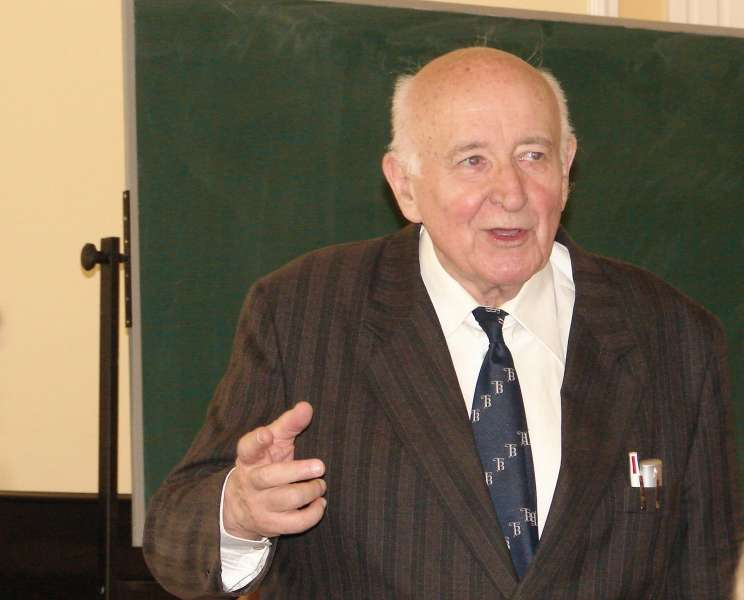
\includegraphics[height=\the\HauteurDesPhotos]{Kurzweil}&
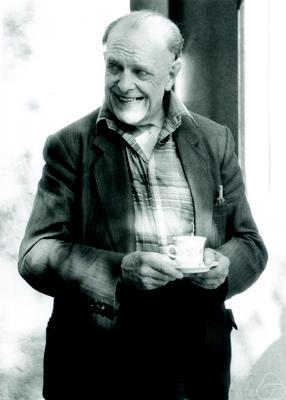
\includegraphics[height=\the\HauteurDesPhotos]{Henstock}\\
Kurzweil&Henstock%
\end{tabular}}
\medskip
\ImageAGauche{%
\textcolorgris{Dans les années 50 a été mise au point l'intégrale de Kurzweil-Henstock\index[aut]{Kurzweil (Jaroslav), 1926-, Tchèque}\index[aut]{Henstock (Ralph), 1923-2007, Anglais} (ou KH-intégrale, ou intégrale de jauge) à partir de celle de Riemann. On retravaille un peu les sous-intervalles et les points de calcul de la fonction: chaque point est appelé «marque» et l'on parle de «subdivision marquée» (pour plus de détails, chercher «lemme de Cousin». Pierre Cousin\index[aut]{Cousin (Pierre), 1867-1933, Français} était un étudiant de Henri Poincaré).\index[aut]{Poincaré (Henri), 1854-1912, Français}\\ 
\indent Sans faire appel à la théorie de la mesure, on dispose alors d'une intégrale aussi puissance que celle de Lebesgue (mais moins générale, car définie uniquement sur~$\RR$). Et on dispose même d'un très beau résultat: toute fonction dérivée est intégrable, et il n'est pas nécessaire d'introduire la notion d'intégrale impropre. L'intégrale de Lebesgue peut alors être introduite comme un cas particulier de cette intégrale.}}
\end{histoire}\colorblack




\medskip
\section{Présentation des espaces de Lebesgue~$L^p$}\index{espace!de Lebesgue}\index[aut]{Lebesgue (Henri-Léon), 1875-1941, Français}

\begin{definition}[Ensemble des fonctions mesurables]
Soit~$(E,\mathcal{A},\mu)$ un espace mesuré.
Si~$\colorred p\in\intfo{1}{+\infty}$, on note~$\colorblue \mathcal{L}^p=\mathcal{L}^p(E,\mathcal{A},\mu)$ l'ensemble de toutes
les fonctions mesurables sur~$(E,\mathcal{A})$, à valeurs dans~$\RR$, telles que la fonction
$|f|^p$ soit~$\mu$-intégrable.

Si~$f\in\mathcal{L}^p$, on pose:
\begin{equation}\|f\|_p=\left(|f|^p\dd\mu\right)^{1/p} \end{equation}
\end{definition}

\begin{theoreme}
Chaque espace~$\mathcal{L}^p$ est un espace vectoriel.
\end{theoreme}

\begin{definition}[Espace~$L^p$]
Soit~$(E,\mathcal{A},\mu)$ un espace mesuré.
Si~$\colorred p\in\intfo{1}{+\infty}$, on note~$\colorblue L^p=L^p(E,\mathcal{A},\mu)$ l'ensemble des
classes d'équivalence des fonctions de~$\mathcal{L}^p$ pour la relation d'équivalence
«égualité~$\mu$-presque partout».

Si~$f\in L^p$, on note~$\|f\|_p$ la valeur commune des~$\| g\| _p$ pour toutes les fonctions~$g$
appartenant à la classe de~$f$.
\end{definition}

De manière équivalente, on peut également définir~$L^p$ comme étant le quotient de~$\mathcal{L}^p$ par la relation d'équivalence «égalité~$\mu$-presque partout».

\medskip
Il est clair que chaque espace~$L^p$ est plus exactement une classe d'équivalence obtenu en identifiant les fonctions qui ne diffèrent que sur un ensemble négligeable.
Ainsi, si~$f\in L^p$, on appelle «représentant» de~$f$, toute fonction mesurable~$g\in\mathcal{L}^p$ qui appartient à la classe d'équivalence de~$f$.

Comme, par construction, deux représentant d'une même classe auront la même intégrale, on
appelle (abusivement, mais sans confusion) tout~$f\in L^p$ une fonction de~$L^p$ et non pas une classe d'équivalence ou un représentant de la classe d'équivalence.
En d'autres termes, on identifie une classe à l'un quelconque de ses représentants.

\medskip
\textcolorgris{En toute généralité, on aura bien remarqué que les définitions précédentes sont liées à la mesure~$\mu$ utilisée. Si l'on considère simultanément deux mesures~$\mu$ et~$\nu$, les classes d'équivalences ne sont pas les mêmes respectivement à chacune de ces mesures, et l'identification d'une classe à l'un quelconque de ses représentant ne peut plus se faire.}

\begin{theoreme}
Chaque espace~$L^p$ est un espace vectoriel.
\end{theoreme}

Un espace~$L^p$ est un espace vectoriel (des classes) de fonctions dont la puissance d'exposant~$p$ est
intégrable au sens de Lebesgue, où~$p$ est un nombre réel strictement positif.
Le passage à la limite de l'exposant aboutit à la construction des espaces~$L^\infty$ des fonctions
bornées.

\medskip
\begin{theoreme}
Chaque espace~$L^p$ est un espace de Banach lorsque son exposant~$p$ est~$\ge 1$.
\end{theoreme}

\begin{theoreme}
Lorsque~$0 < p < 1$, l'intégrale définit une quasi-norme qui en fait un espace complet.
\end{theoreme}


\medskip
\begin{definition}[Exposants conjugués]\index{exposant conjugué!de Lebesgue}
Soient~$p$ et~$q\in [1,+\infty]$. On dit que~$p$ et~$q$ sont des exposants conjugués si:
\begin{equation}\colorred\dfrac1p + \dfrac1q = 1 \end{equation}
\end{definition}

\begin{theoreme}
Soient~$p$ et~$q$ des exposants conjugués, alors il existe une \textcolorblue{dualité} entre les espaces d'exposants~$p$ et~$q$.
\end{theoreme}
\colorgris
Il suffit en effet de considérer, à~$g\in L^q$ fixé (de mesure~$\mu$), l'application~$\varphi_g: f\mapsto \int fg\dd\mu$. Cette dernière
définie une forme linéaire continue sur~$L^p$.
\colorblack

\medskip
\section{Construction de~$L^p$}

On considère~$\Omega$ un ouvert de~$\RR^n$.
Les fonctions~$f$ seront considérées de~$\Omega$ dans~$\RR$ ou~$\CC$.

\medskip
On appelle~$\colorblue L^p \colorblack= L^p_M(\Omega,\CC)$ pour~$p<\infty$
l'espace des fonctions~$f$ mesurables, de~$\Omega \rightarrow \CC$, telles que
$\mu(|f|^p)<\infty$ où~$\mu$ est une mesure sur~$\Omega$.

\medskip
Comme une fonction s'annulant presque partout est d'intégrale nulle, on peut définir
l'espace~$L^p(X, \mathcal{A}, \mu)$ comme le quotient de l'espace des fonctions~$p$ intégrables
$L^p(X, \mathcal{A}, \mu)$ par le sous-espace vectoriel des fonctions presque nulles.

\textcolorgreen{Ce quotient identifie donc les fonctions qui sont presque partout égales,
autrement dit qui ne diffèrent que sur un ensemble de mesure nulle.}

\medskip
\begin{definition}[Norme~$L^p$]
Pour~$p<\infty$, on appelle \textcolorblue{norme~$L^p$} et on note~$\|\cdot\|_p$,
l'application définie par~$\|f\|_p=\left(\dint_\Omega |f|^p\right)^{1/p}$.
\end{definition}

Sur~$\RR$, cela donne:~$\|f\|_p=\left(\dint_a^b |f(t)|^p\dd t\right)^{1/p}$.

Sur un espace mesuré~$(X, \mathcal{A}, \mu)$ et à valeurs réelles ou complexes:~$\|f\|_p=\left(\dint_X |f|^p\dd\mu\right)^{1/p}$.

\medskip
\begin{theoreme}
Si l'espace~$X$ est fini et est muni d'une mesure finie~$\mu(X)<\infty$, alors tous les espaces~$L^p$
(resp.~$\mathcal{L}^p$), pour~$1\le p\le \infty$ sont les mêmes.
\end{theoreme}

\begin{definition}[Espace des suites]
Soit~$X=\NN$ muni de sa tribu~$\mathcal{A}=\mathcal{P}(X)$ et de sa mesure de comptage~$\mu$.
On note~$\ell^p$ l'espace~$L^P(X,\mathcal{A},\mu)=\mathcal{L}^p(X,\mathcal{A},\mu)$.
Cet espace est l'espace des suites~$(u_n)_{n\in\NN}$ telles que:
\begin{equation}
\left\{
\begin{array}{lll}
\text{Si } 1\le p<\infty: &\quad \dsum_n |u_n|^p<\infty, &\quad \text{ et } \|u_n\|_p=\left(\dsum_n|u_n|^p\right)^{1/p}\\
\text{Si } p=\infty: &\quad \sup_n |u_n|^p<\infty, &\quad \text{ et } \|u_n\|_\infty=\sup_n|u_n|
\end{array}
\right.
\end{equation}
\end{definition}

\medskip
\section{Espace~$L^0$}
L'espace~$L^0$ est l'ensemble des fonctions mesurables.
$L^0$ est l'espace obtenu en quotientant~$L^0$ par les fonctions nulles.

\medskip
Soit~$\varphi$ une fonction mesurable strictement positive et~$\mu$-intégrable, alors:
\begin{equation}
\rho(f,g)=\dint \frac{\|f-g\|}{1+\|f-g\|} \varphi \dd\mu
\end{equation}
définit une distance sur~$L^0$ qui redonne la topologie de la convergence en mesure.

\begin{theoreme}
Muni de cette distance, l'espace~$L^0$ est complet.
\end{theoreme}

\medskip
Rappel: la notion de convergence (de suite) est une propriété topologique et non
métrique (l'écriture avec les~$\varepsilon$ n'est que la traduction métrique
de l'écriture topologique avec les boules).

\medskip
\section{Espace~$L^\infty$ et dualité avec~$L^1$}
Dans le cas où l'exposant est infini, on procède de la même manière.

\medskip
L'espace~$L^\infty(X, \mathcal{A}, \mu)$ est défini comme l'espace vectoriel des fonctions
$\mu$-essentiellement bornées (i.e. des fonctions bornées presque partout).

L'espace~$L^\infty(X, \mathcal{A}, \mu)$ est l'espace vectoriel quotient de~$L^\infty(X, \mathcal{A}, \mu)$
par la relation d'équivalence «$f \sim g$» ssi «$f$ et~$g$ sont égales presque partout».

\begin{theoreme}
L'espace dual de~$L^1$ est~$L^{\infty}$ mais l'espace dual de~$L^{\infty}$ contient strictement~$L^1$.
\end{theoreme}

\medskip
\section{Espace~$L^2$}

Par définition, si~$\Omega$ est un ouvert donné de~$\RR^n$, $L^2(\Omega)$ est l'espace des
fonctions (réelles ou complexes) qui sont de carré intégrable au sens de l'intégrale de Lebesgue.

\medskip
\begin{theoreme}
\textcolorred{L'espace~$L^2$ est un espace de Hilbert lorsqu'il est muni du produit scalaire:
\begin{equation}(f,g) = \dint_{\Omega} f \bar g \,\dd\mu\end{equation}}\index{produit scalaire!de~$L^2$}
\end{theoreme}

\medskip
La formule des exposants conjugués conduit dans le cas~$p=2$, à~$q=2$, i.e.
que \textcolorred{$L^2$ s'identifie à son dual.}

\textcolorgris{Si l'on reprend la remarque précédente sur la dualité, cela devient dans~$L^2$ (et dans tout espace de
Hilbert~$H$): en associant à tout~$v\in H$ l'application~$\varphi_v(u)=\langle u,v\rangle$, on peut identifier l'espace
de Hilbert~$H$ a son dual~$H'$.}

\medskip
\textcolorgreen{Comme mentionné, l'intérêt d'avoir un espace de Hilbert est de disposer d'un produit scalaire, donc
de pouvoir décomposer un vecteur. Ce que l'on retrouve dans le théorème suivant, vrai dans~$L^2$ ainsi que dans
tout espace de Hilbert:}

\begin{theoreme}
Tout vecteur~$u$ d'un espace de Hilbert~$H$ se décompose de manière unique en une somme~$u=v+w$ avec
$v\in K$ et~$w\in K^\bot$, et les sous-espaces~$K$ et~$K^\bot$ sont supplémentaires dans~$H$.
\end{theoreme}

On rappelle que:
\begin{definition}[Orthogonal d'une partie]
$K$ étant une partie de~$H$, on note~$K^\bot$ l'ensemble des vecteurs~$u\in H$ qui sont orthogonaux à tous les
vecteurs de~$K$.
\end{definition}

\begin{theoreme}
L'orthogonal~$K^\bot$ de toute partie de~$K$ d'un espace de Hilbert~$H$ est un sous-espace vectoriel fermé de
$H$, donc lui-même un espace de Hilbert.

On a~$(K^\bot)^\bot = K$.
\end{theoreme}

\medskip
\section{Compléments}

Commençons par quelques exemples ultra classiques:
\begin{itemize}
  \item La fonction~$1/\sqrt{x}$ est~$L^1$ mais pas~$L^2$.
  \item La fonction~$1/|x|$ est~$L^2$ mais pas~$L^1$.
  \item La fonction~$\mathrm{e}^{-|x|}/\sqrt{|x|}$ est~$L^1$ mais pas~$L^2$
\end{itemize}

\medskip
Poursuivons par quelques inégalités bien utiles.

\begin{theoreme}[Inégalité de Minkowski]\index[aut]{Minkowski (Hermann), 1864-1909, Allemand}
Soient~$p\in[1,\infty]$, et~$f$ et~$g$ dans~$L^p$, alors on a:
\begin{equation}\|f+g\|_p\le\|f\|_p+\|g\|_p\end{equation}
\end{theoreme}

\begin{theoreme}[Inégalité de Hölder]\index[aut]{Hoelder@Hölder (Otto Ludwig), 1859-1937, Allemand}
Soient~$p$, $q$ et~$r$ des nombres de~$[1,\infty]$ vérifiant
$\dfrac1p+\dfrac1q=\dfrac1r$ (avec la convention~$1/\infty=0$).
Si~$f\in L^p$ et~$g\in L^q$, alors le produit~$fg\in L^r$, et on a:
\begin{equation}\|fg\|_r\le\|f\|_p\|g\|_q\end{equation}
\end{theoreme}

L'inégalité de Hölder conduit au théorème suivant:
\begin{theoreme}
Si~$\mu$ est une mesure finie et si~$1\le p\le q\le \infty$, on a:
\begin{equation}L^q\subset L^p\end{equation}
\end{theoreme}

\medskip
Terminons en revenons un peu à nos fonctions continues~$C^k$, et plus précisément sur les fonctions continues à support compact
dans un ouvert~$\Omega$ mesurable de~$\RR^n$ (voir la définition~\ref{Def-Cc} page \pageref{Def-Cc}).
On dispose des résultats de \textcolorblue{densité} suivants:
\begin{itemize}
  \item L'espace~$C_c^0(\Omega)$ des fonctions continues à support compact est dense dans~$L^p(\Omega)$ pour~$1\le p<\infty$
	(mais n'est pas dense dans~$L^\infty(\Omega)$)

	\colorgris Dans le cas~$p=1$, cela se traduit par: 	$ \forall f\in L^1(\Omega), \forall\varepsilon>0, \exists g\in C_ c^0(\Omega), \text{ tel que }
	  \|f-g\|_{L^1(\Omega)}\le\varepsilon$ \colorblack

  \item L'espace~$C_c^\infty(\Omega)$ des fonctions infiniment dérivables à support compact est dense dans~$L^p(\Omega)$ pour~$1\le p<\infty$
	(mais n'est pas dense dans~$L^\infty(\Omega)$)
  \item L'espace~$C_c^\infty(\Omega)$ est dense dans le sous espace de~$L^\infty(\Omega)$ des fonctions bornées qui tendent vers 0 en l'infini.
  \item L'ensemble des fonctions continues à support compact de~$L^p(\RR^n)$ est dense dans~$L^p(\RR^n)$, pour~$ p\neq \infty$. 
\end{itemize}

\textcolorgreen{Les arguments de densité ont une importance pratique dans certaines démonstrations:}
si l'on doit démontrer qu'une propriété est vérifiée sur~$L^p(\Omega)$, alors on peut commencer par montrer que cette propriété est 
vraie sur~$C_c^\infty(\Omega)$, avant de passer à la limite en utilisant l'argument de densité:
«$C_c^\infty(\Omega)$ est dense dans~$L^p(\Omega)$».

\medskip
L'espace~$C_c^{\infty}(\Omega)$ est également noté~$\mathcal{D}(\Omega)$ et appelé espace des fonctions tests. 
Les distributions sont définies comme les éléments de~$\mathcal{D}'(\Omega)$, dual topologique de~$\mathcal{D}(\Omega)$, 
muni d'une topologie adéquate.
Nous allons les aborder dès a présent, au chapitre~\ref{Ch-Sobo}.
